\documentclass[12pt]{amsart}

\addtolength{\hoffset}{-2.25cm}
\addtolength{\textwidth}{4.5cm}
\addtolength{\voffset}{-2.5cm}
\addtolength{\textheight}{5cm}
\setlength{\parskip}{0pt}
\setlength{\parindent}{15pt}

\usepackage[export]{adjustbox}
\usepackage{listings}
\usepackage{amsthm}
\usepackage{amsmath}
\usepackage{amssymb}
\usepackage[colorlinks = true, linkcolor = black, citecolor = black, final]{hyperref}

\usepackage{graphicx}
\usepackage{multicol}
\usepackage{ marvosym }
\usepackage{wasysym}
\usepackage{tikz}
\usetikzlibrary{patterns}

\newcommand{\ds}{\displaystyle}
\DeclareMathOperator{\sech}{sech}


\setlength{\parindent}{0in}

\pagestyle{empty}

\begin{document}

\thispagestyle{empty}

{\scshape COSC 525} \hfill {\scshape \large Project 2: Convolutional Neural Network} \hfill {\scshape 2021-03-07}

\smallskip 

{University of Tennessee} \hfill { Su-Ann Chong}

\smallskip

\hrule

\bigskip
\section{Introduction}
% A short introduction to the problem 
Building off the artifical neural network library created in Project 1, several modifications are introduced to build a convolutional neural network. Specifically, several classes are introduced, namely

$$ \texttt{ConvolutionalLayer} $$
$$  \texttt{MaxPoolingLayer} $$
$$ \texttt{FlattenLayer} $$  

\bigskip

An additional method \texttt{addLayer} is introduced in the \texttt{NeuralNetwork} class to allow for a variable number of layers in the neural network with different layer types. \\

% This library can handle inputs with variable input size ($w \times h$) and number of channels, $c$ and kernel with variable kernel size ($kw \times kh$) and number of kernels, $k$.

In this project, the convolution layer is restricted to 2-dimensional convolution with a stride of 1 and padding is set to 'valid'. The max pooling layer is also restricted to 2-dimensional with the stride is always the same as the filter size and no padding is needed. \\

The options for activation function are logistic function (sigmoid) and linear function. The options for loss function are mean squared error and binary cross entropy. \\

Code examples are run using the TensorFlow with the keras API (tf.keras) to validate the correctness of the convolutional neural network library. The input, output, weights and bias are generated using \texttt{parameter.py} with a random seed specified so the results are reproducible. 

\section{Assumptions/choices made}
\begin{itemize}
	% \item The convolution layer is restricted to 2-dimensional convolution with a stride of 1 and padding is set to 'valid'.
	% \item The max pooling layer is also restricted to 2-dimensional with the stride is always the same as the filter size and no padding is needed.
	% \item All weights are randomly initialized if not given during initialization of the model.
	% \item The options for activation function are logistic function (sigmoid) and linear function.
	% \item The options for loss function are mean squared error and binary cross entropy
	\item The input for each layer type (except for the fully connected layer) has a dimension of $(w, h, c)$ where $w$ is the width of the input, $h$ is the height of the matrix and $c$ is the number of input channels.
	\item The fully connected layer accepts an input with a dimension of $(n,m)$, where $n$ is the number of neurons in the fully connected layer and $m$ is the size of the flattened input.
	\item The kernel for each convolutional layer has a dimension of $(k, kw, kh)$ where $k$ is the number of kernel, $kw$ is the width of the kernel and $kh$ is the height of the kernel. 
	\item The argument of the \texttt{addLayer} method accepts 4 layer types, namely:
	 \begin{itemize}
	 	\item "Conv2D" 		 : 2-dimensional convolutional layer 
	 	\item "Dense"  		 : fully connected layer 
	 	\item "MaxPooling2D" : 2-dimensional max pooling layer
	 	\item "Flatten" 	 : flatten layer 
	 \end{itemize}
\end{itemize}

\section{Problems/Issues}
There is a slight discrepancy between the solution of the project code and the solution of the TensorFlow keras API. This may be due to round-off errors.

\section{How to run the code}
You can run the project code with examples using the following command:
\begin{lstlisting}[language=bash]
$ python project2.py [example1|example2|example3]
\end{lstlisting}

You can choose one example to run with either example1, example2 or example3. \\

To run the code examples with the TensorFlow keras API, use the following commands:
\begin{lstlisting}[language=bash]
$ python tensorflowtest_example1.py
$ python tensorflowtest_example2.py
$ python tensorflowtest_example3.py
\end{lstlisting}

\section{Results}
The results from each run of one-step backpropagation using the project code are compared to the results from one run of Tensorflow keras API with the same input paramters.\\

The code examples are:
\begin{itemize}
\item Example 1: Run a network with a 5$\times$5 input, one 3$\times$3 convolutional layer with a single kernel, a flatten layer and a single neuron for the output.

\item Example 2: Run a network with a 7$\times$7 input, one 3$\times$3 convolutional layer with two kernels, another 3$\times$3 convolutional layer with a single kernel, a flatten layer and a single neuron for the output.

\item Example 3: Run a network with an 8$\times$8 input, one 3$\times$3 convolutional layer with two kernels, a 2$\times$2 max pooling layer, a flatten layer and a single neuron for the output. 
\end{itemize}

\begin{figure}[h]
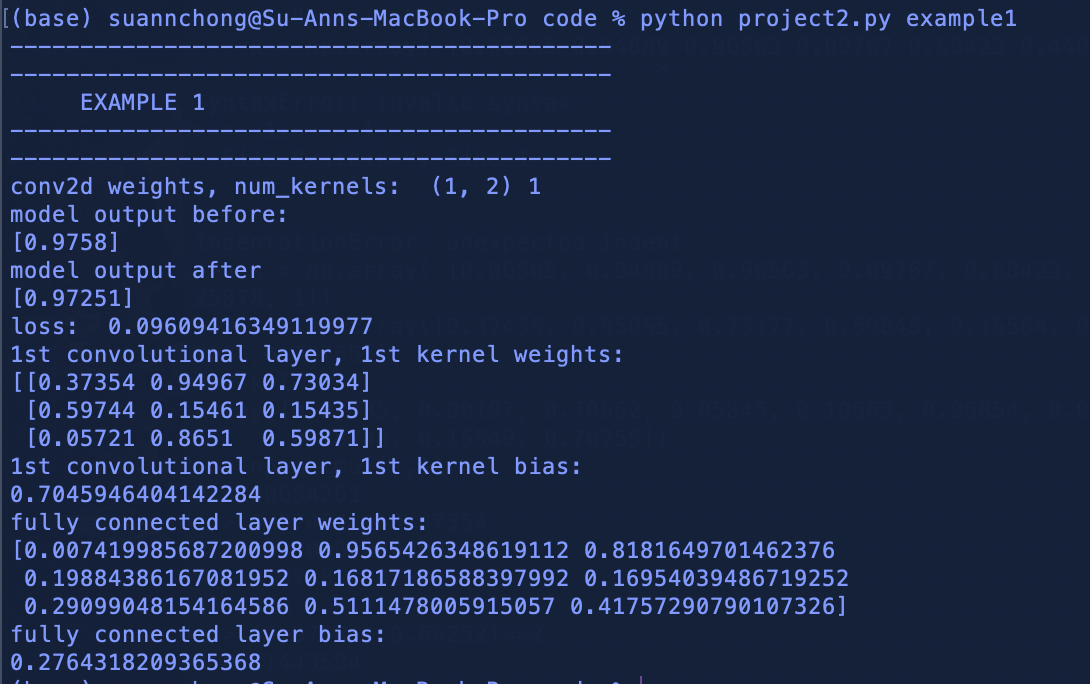
\includegraphics[height=0.33\textheight, width=0.49\textwidth]{ex1_proj.png}
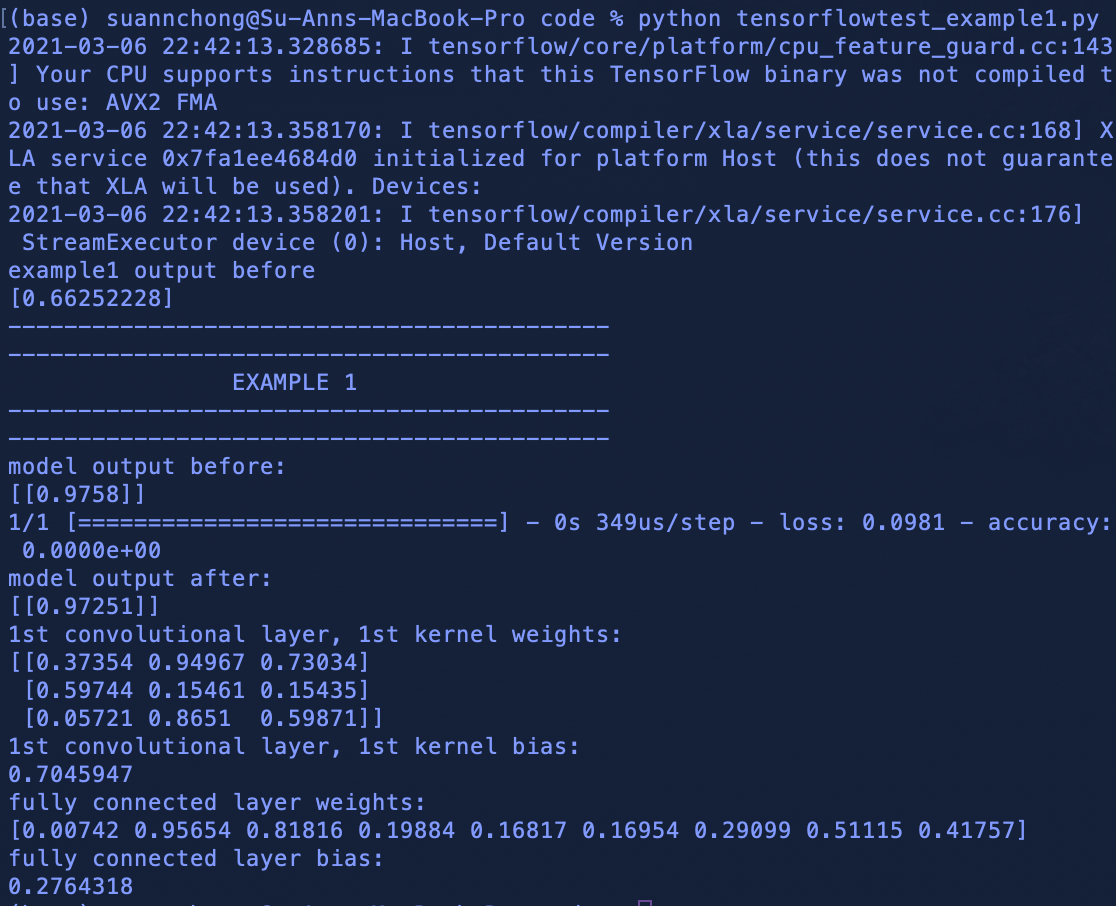
\includegraphics[height=0.33\textheight, width=0.49\textwidth]{ex1_tf.png}
\caption{Screenshots of the project solution (on left) and the TensorFlow keras API solution (on right) for Example 1.}
\end{figure}

% \subsection{Example 2}

\begin{figure}[h]
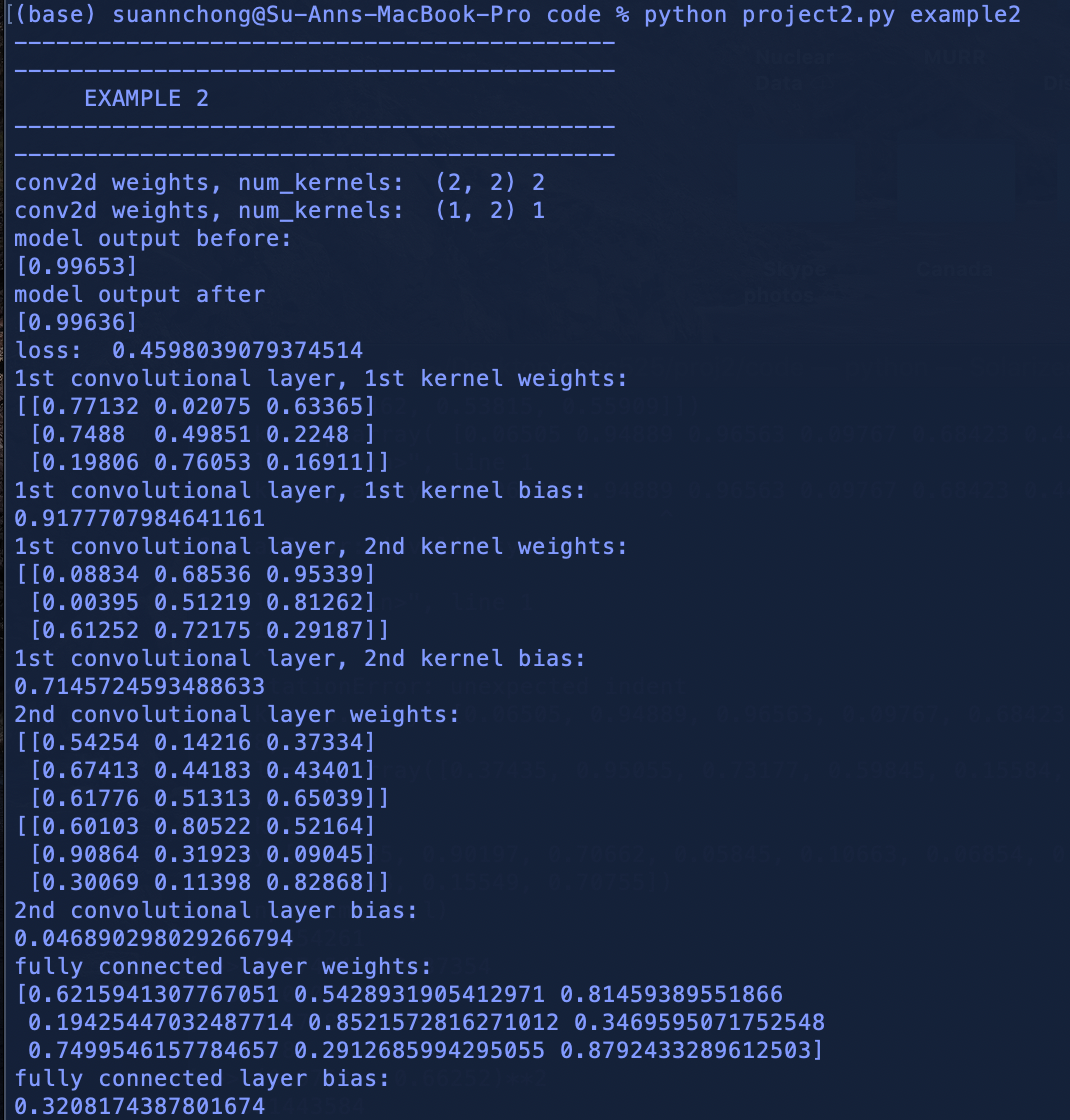
\includegraphics[height=0.33\textheight, width=0.49\textwidth]{ex2_proj.png}
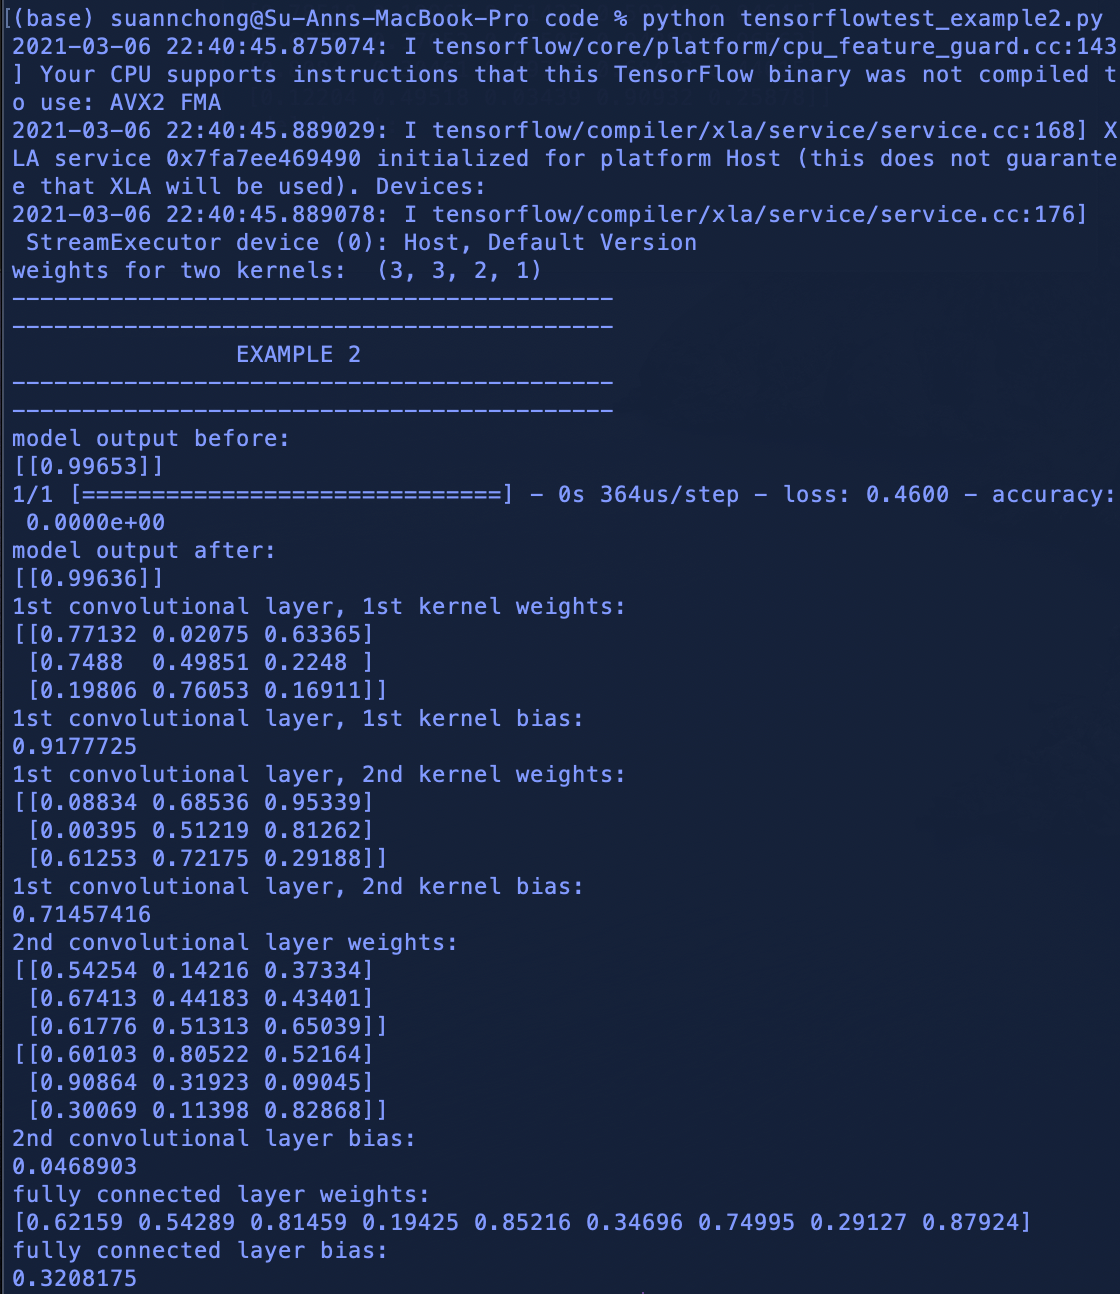
\includegraphics[height=0.33\textheight, width=0.49\textwidth]{ex2_tf.png}
\caption{Screenshots of the project solution (on left) and the TensorFlow keras API solution (on right) for Example 2.}
\end{figure}

% \subsection{Example 3}

\begin{figure}[h!]
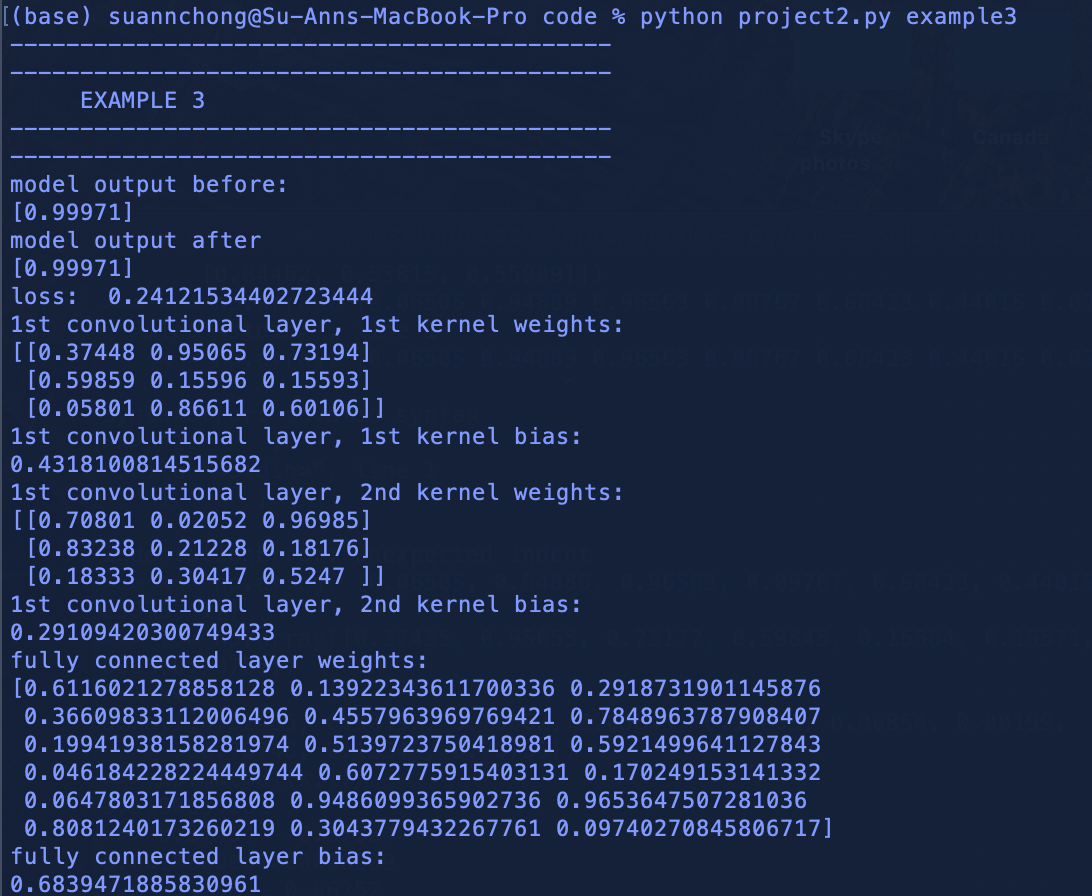
\includegraphics[height=0.33\textheight, width=0.49\textwidth]{ex3_proj.png}
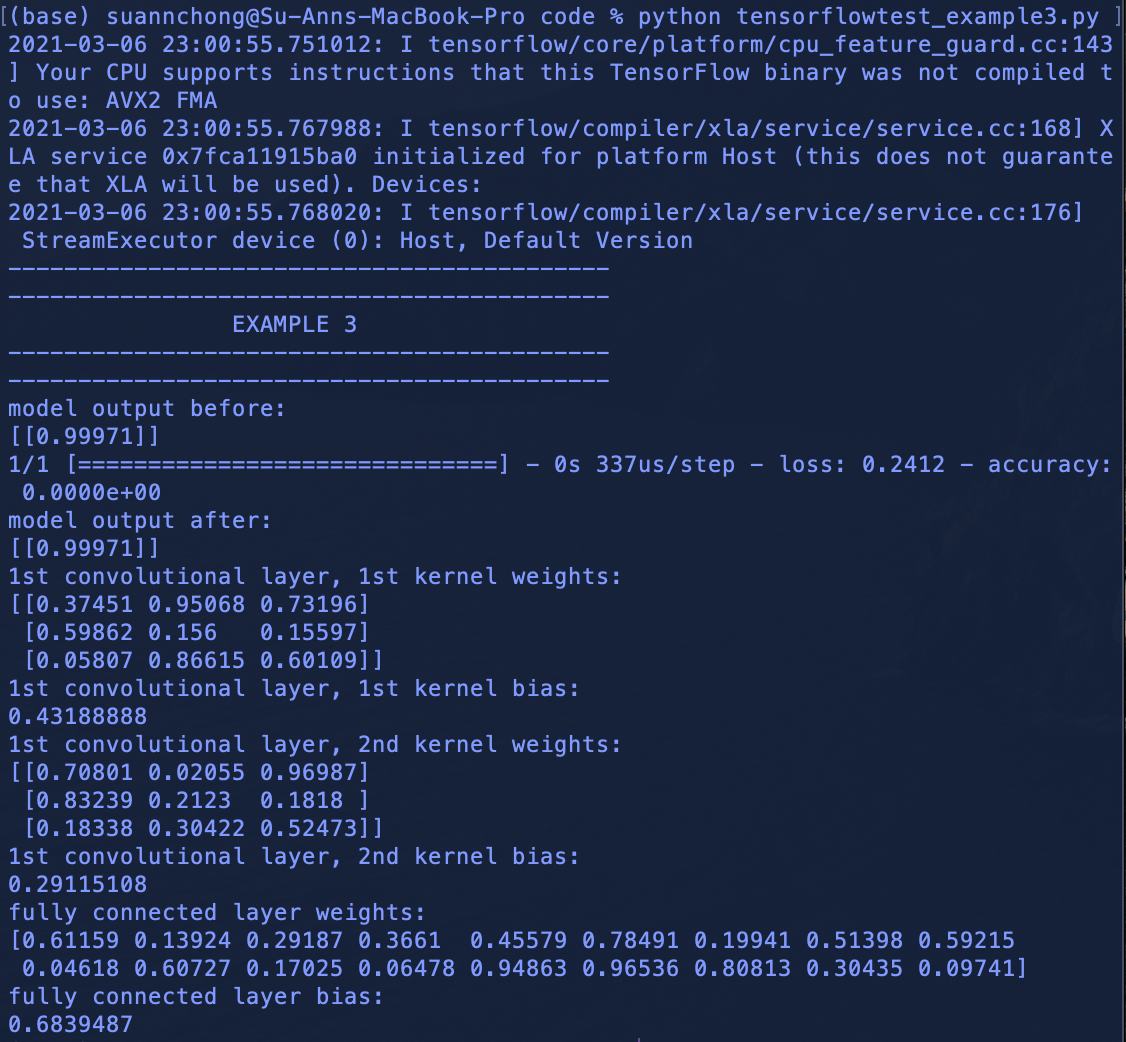
\includegraphics[height=0.33\textheight, width=0.49\textwidth]{ex3_tf.png}
\caption{Screenshots of the project solution (on left) and the TensorFlow keras API solution (on right) for Example 3.}
\end{figure}

\end{document}